\section{Triển khai hệ thống}
\subsection{Triển khai các dịch vụ}
% \lipsum[1]

\subsection{Tổng quan các Microservice của hệ thống}

\begin{figure}[H]
\centering
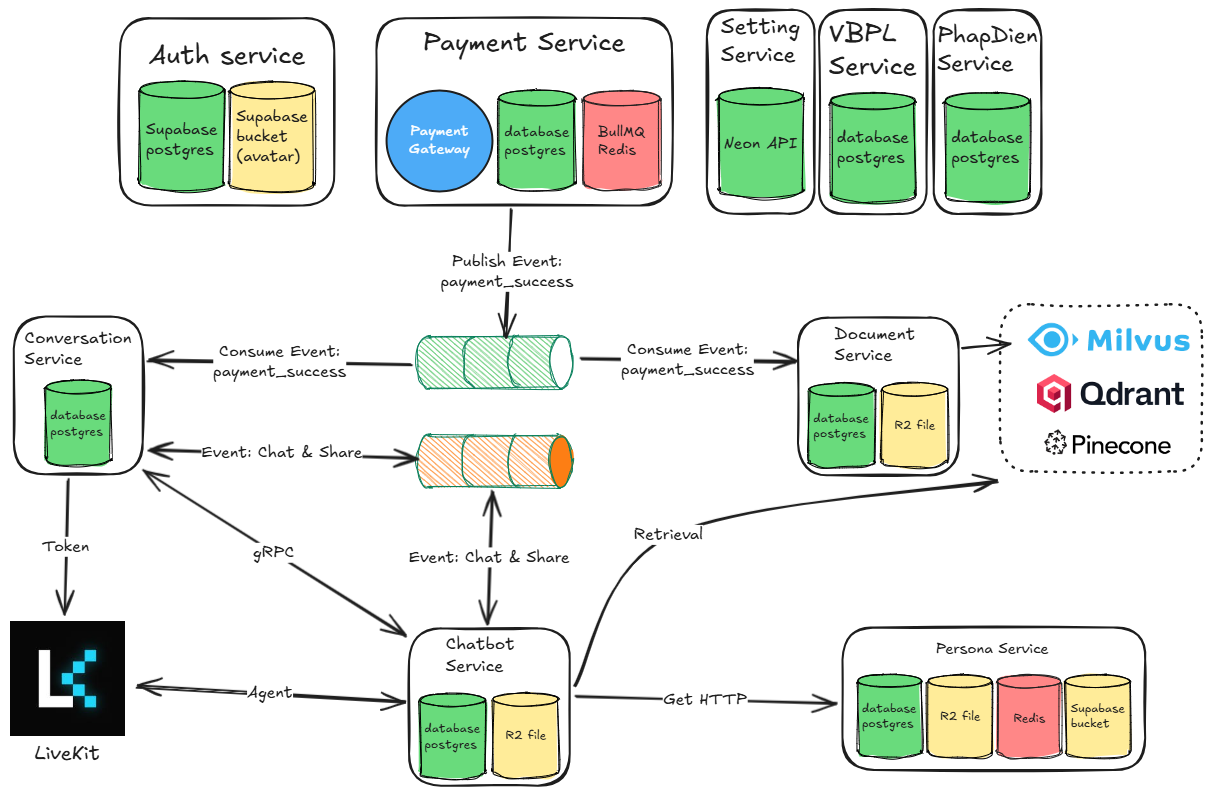
\includegraphics[width=0.85\textwidth]{pictures/Microservice-all.excalidraw.png}
\caption{Sơ đồ tổng quan các Microservice}
\label{fig:microservice-all}
\end{figure}

Tất cả các dịch vụ đều dùng \url{https://[PROJECT_REF].supabase.co/auth/v1/.well-known/jwks.json} để xác thực thông tin JWT của người dùng.

Tất cả các dịch vụ đều dùng cơ sở dữ liệu Postgres của Neon để làm cơ sở dữ liệu riêng theo đúng mẫu cơ sở dữ liệu cho mỗi dịch vụ (database per service pattern). Mỗi dịch vụ sẽ sở hữu và quản lý hoàn toàn cơ sở dữ liệu của riêng nó.

\begin{figure}[H]
\centering
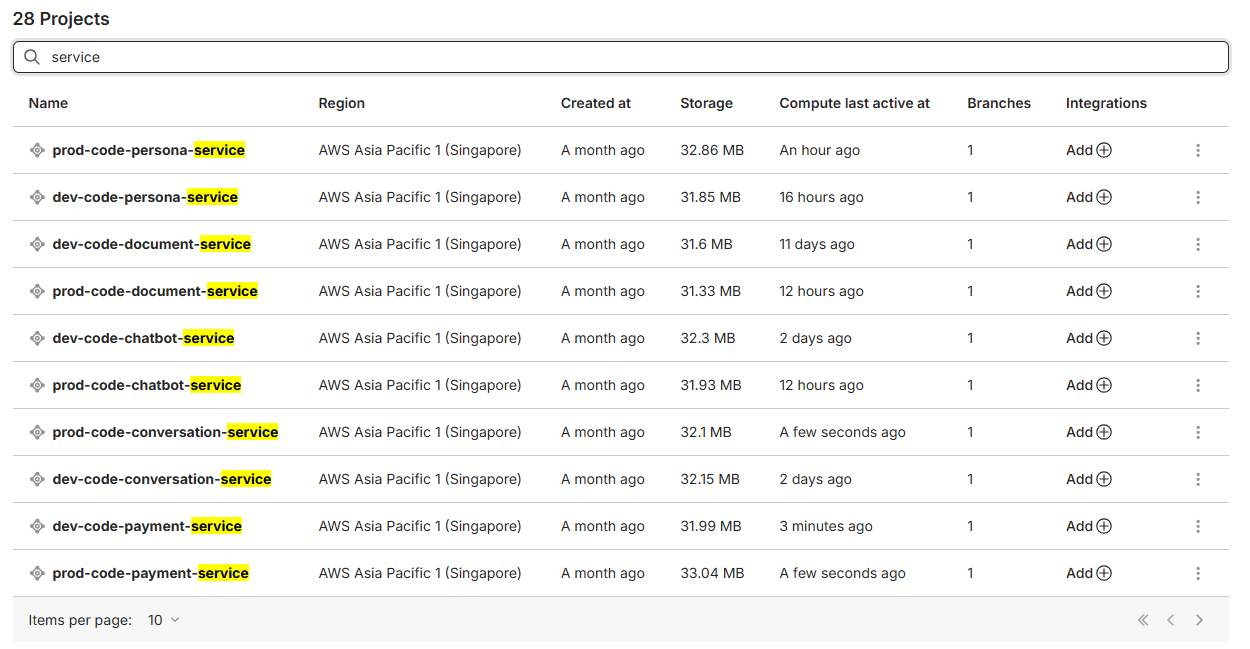
\includegraphics[width=0.85\textwidth]{pictures/neon-database-all.png}
\caption{Bảng điều khiển cơ sở dữ liệu Neon}
\label{fig:neon-database-all}
\end{figure}

Các dịch vụ ngoại trừ auth và setting được cấu hình trong Kong API Gateway đơn giản chỉ cần tạo Service và Route để định tuyến request. Dịch vụ auth và setting sẽ được mô tả chi tiết về cách cấu hình trong Kong API Gateway trong nội dung trình bày của chính dịch vụ đó.

Trang thống kê thông tin đường ống dữ liệu (Data Pipeline) dành cho quản trị viên (ADMIN) có tần suất truy vấn thấp nên sẽ được triển khai trên Vercel.

\begin{figure}[H]
\centering
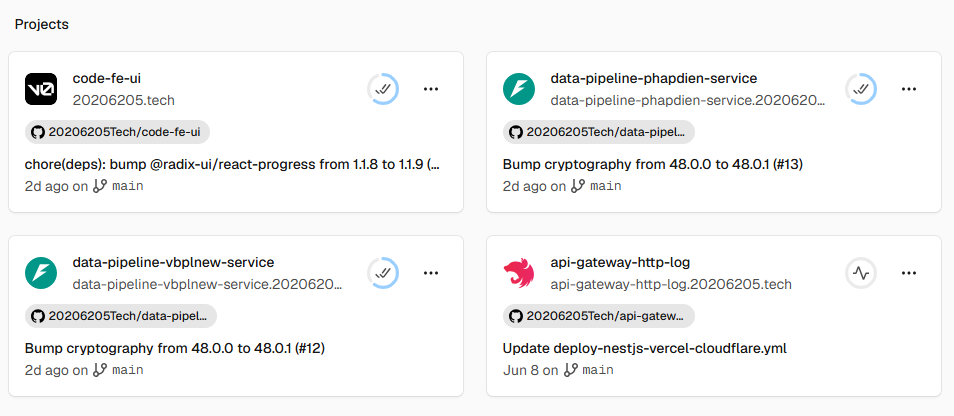
\includegraphics[width=0.85\textwidth]{pictures/vercel-project.png}
\caption{Dự án trên Vercel}
\label{fig:vercel-project}
\end{figure}

Các dịch vụ NestJS sử dụng Codecov để theo dõi độ bao phủ kiểm thử (test coverage).

\begin{figure}[H]
\centering
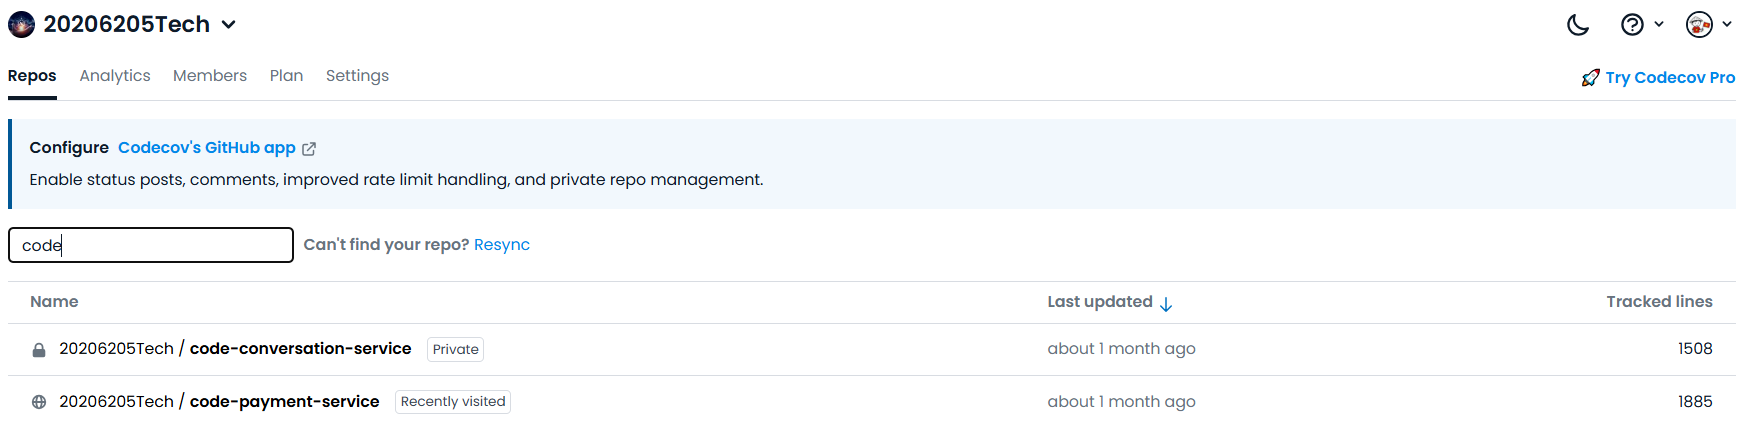
\includegraphics[width=0.85\textwidth]{pictures/test-codecov.png}
\caption{Thống kê độ bao phủ kiểm thử trên Codecov}
\label{fig:test-codecov}
\end{figure}

Tích hợp SonarQube để phân tích chất lượng mã nguồn và các lỗ hổng bảo mật.

\begin{figure}[H]
\centering
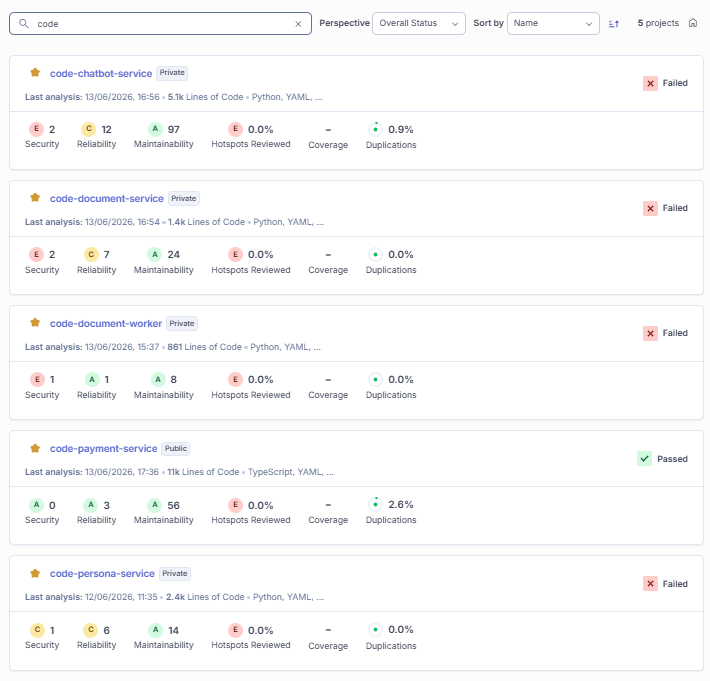
\includegraphics[width=0.85\textwidth]{pictures/sonarqube.png}
\caption{Giao diện phân tích mã nguồn trên SonarQube}
\label{fig:sonarqube}
\end{figure}

\subsubsection{Tracing và Quan sát hệ thống (Observability)}
Hệ thống sử dụng \textbf{OpenTelemetry (OTel)} tích hợp trong tất cả các dịch vụ để tự động thu thập dấu vết phân tán (distributed traces) và gửi dữ liệu về Honeycomb.

Tích hợp Honeycomb để theo dõi vết (distributed tracing) giữa các dịch vụ.

\begin{figure}[H]
\centering
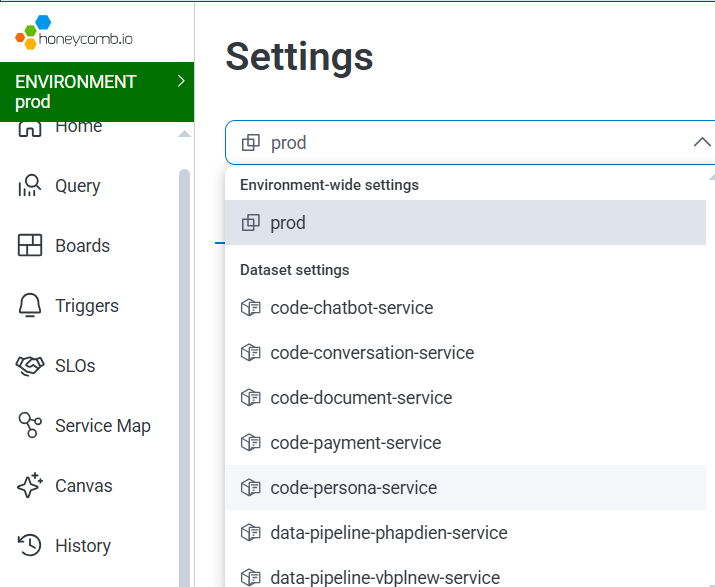
\includegraphics[width=0.85\textwidth]{pictures/tracing.png}
\caption{Giao diện theo dõi vết distributed tracing trên Honeycomb}
\label{fig:tracing}
\end{figure}
